\section{Évaluation de parties}

%label pour referencement
\label{evaluator}

\subsection*{Problématique}

Maintenant que nous sommes capable de jouer des parties de manières indépendantes, il est intéressant de trouver quel couple de graine donne lieu aux parties les plus viables. Pour cela nous avons besoin d'avoir accès aux statistiques de la partie et de jouer un grand nombre de parties avec des graines différentes.

\subsection{Extraction des statistiques d'une partie}

Lorsque qu'un tour est joué, on retourne les statistiques de ce dernier à travers la structure \code{turn\_statistics} qui est ensuite ajouté aux statisques globales de la partie au travers de la structure \code{game\_statistics}.

\begin{lstlisting}[frame=single, caption={Structures pour récupérer les statistiques}]
struct turn_statistics
{
	enum choice choice;
	int used_favor;
	int used_skill;
	int num_picked_tokens;
	int forced_skip;
};


struct game_statistics
{
	int choices[NUM_CHOICE];
	int used_favor;
	int used_skill;
	int num_picked_tokens;
	int forced_skip;
	int nb_turns;
	int result; 
};
\end{lstlisting}

\subsection{Test d'un grand nombre de parties}

Maintenant que l'on peut récupérer les statistiques d'une partie, on teste chaque couple de graines avec 100 graines aléatoires différentes pour récupérer une moyenne des statistiques pour chaque couple que l'on affiche dans la sortie standard sous la forme d'un csv. On peut alors récupérer ces données dans un fichier pour les analyser.

\begin{lstlisting}[frame=single, caption={Affichage des résultats}]
seed_builders;seed_token;choices;used_favor;used_skill;num_picked_tokens;forced_skip;nb_turns;result
1;0;1.85,6.26,1.12;1.27;1.58;12.37;0.01;9.23;0.48
2;0;1.08,7.33,1.10;0.99;1.76;14.23;0.13;9.51;0.35
3;0;1.39,6.66,1.08;0.98;1.22;13.16;0.07;9.13;0.42
4;0;1.47,6.60,1.05;0.98;1.36;13.19;0.05;9.12;0.43
5;0;1.32,6.29,0.96;0.92;1.85;12.11;0.03;8.57;0.53
6;0;1.48,6.74,1.08;0.96;1.04;13.22;0.04;9.30;0.35
7;0;1.84,6.11,1.01;0.97;2.57;12.06;0.02;8.96;0.60
8;0;1.14,6.62,1.06;0.97;1.60;13.03;0.03;8.82;0.55
9;0;1.67,6.57,1.01;0.96;1.23;13.03;0.04;9.25;0.43
...
\end{lstlisting}

\subsection{Analyse des résultats}

A l'aide d'un programme écrit en \code{Python}, on peut visualiser l'influence des différentes graines sur différents paramètres.


\begin{figure}[H]
   \begin{subfigure}[b]{0.3\textwidth}
        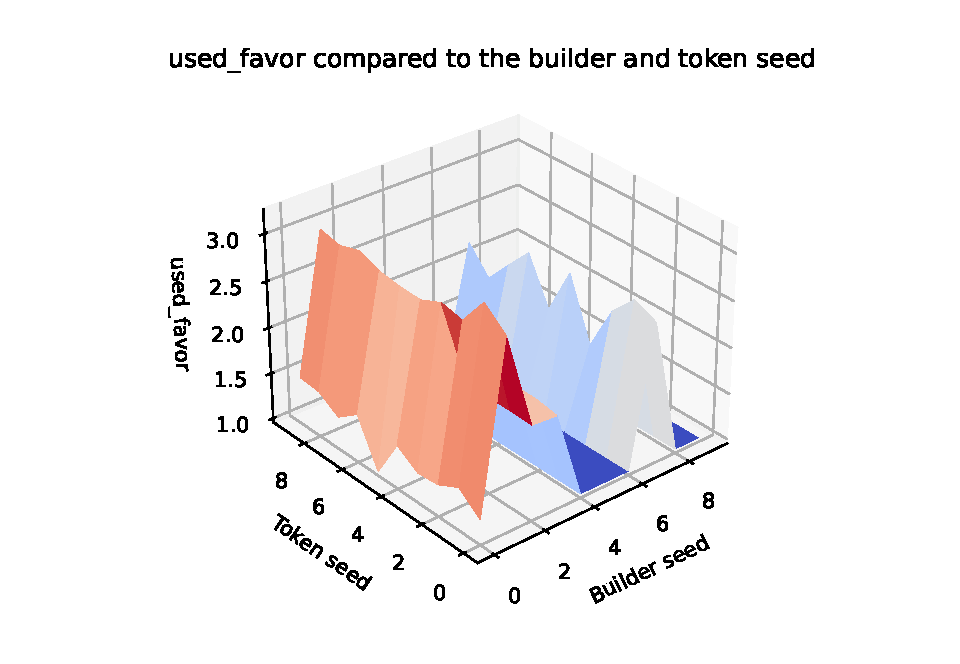
\includegraphics[width=\textwidth]{img/favor.pdf}
    \end{subfigure}
    \begin{subfigure}[b]{0.3\textwidth}
        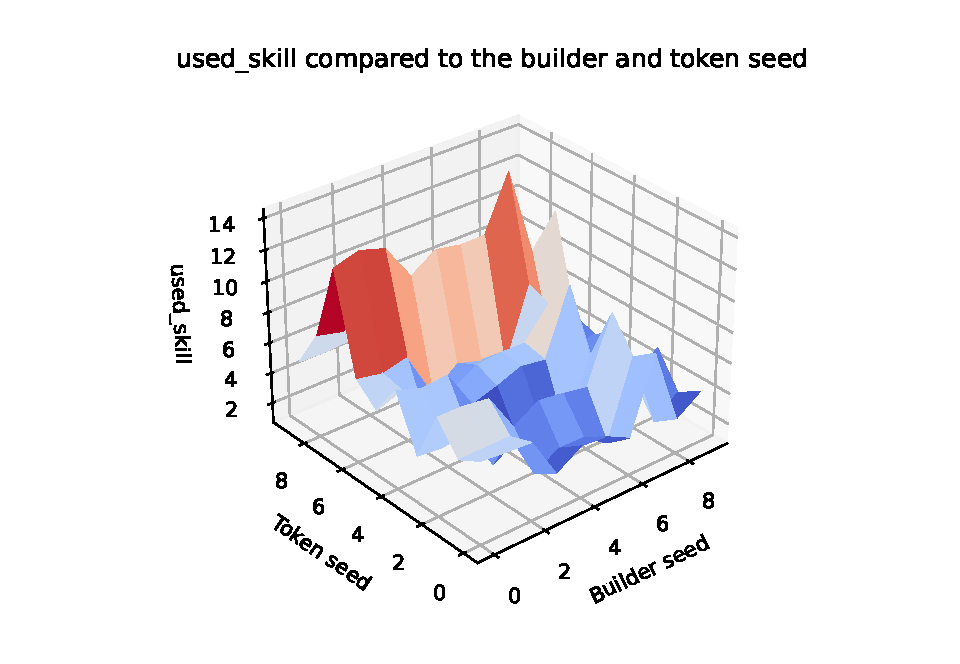
\includegraphics[width=\textwidth]{img/skills.pdf}
    \end{subfigure}
    \begin{subfigure}[b]{0.3\textwidth}
        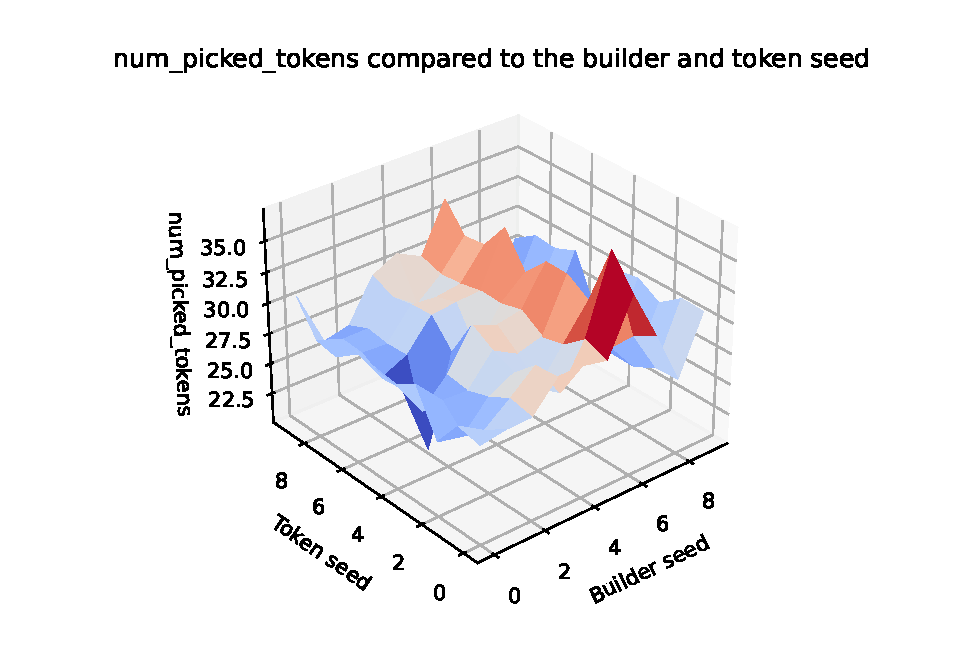
\includegraphics[width=\textwidth]{img/tokens.pdf}
    \end{subfigure} 
    \\
    \begin{subfigure}[b]{0.3\textwidth}
        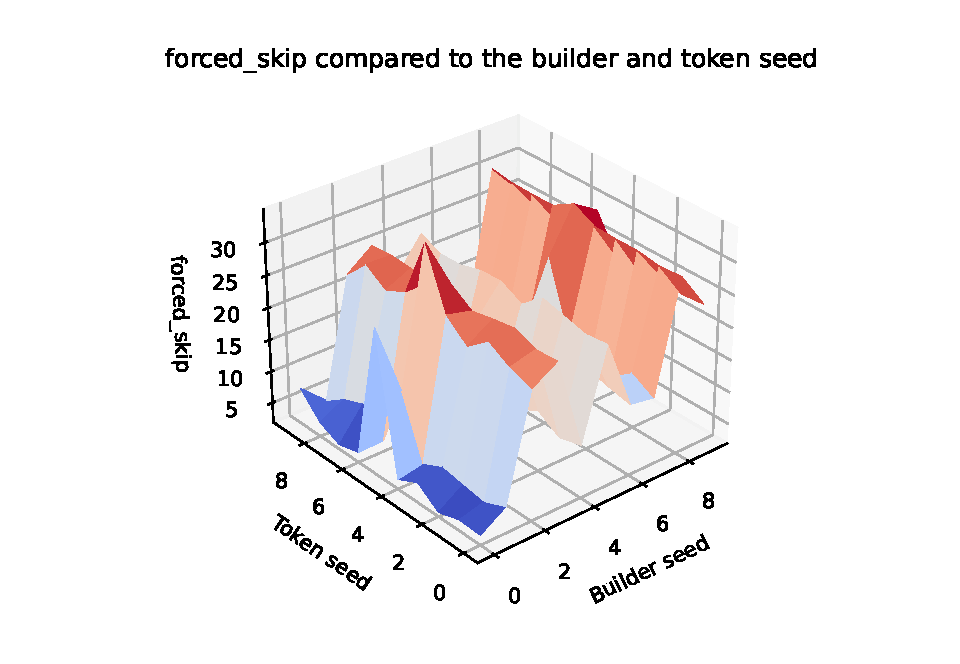
\includegraphics[width=\textwidth]{img/skip.pdf}
    \end{subfigure}
    \begin{subfigure}[b]{0.3\textwidth}
        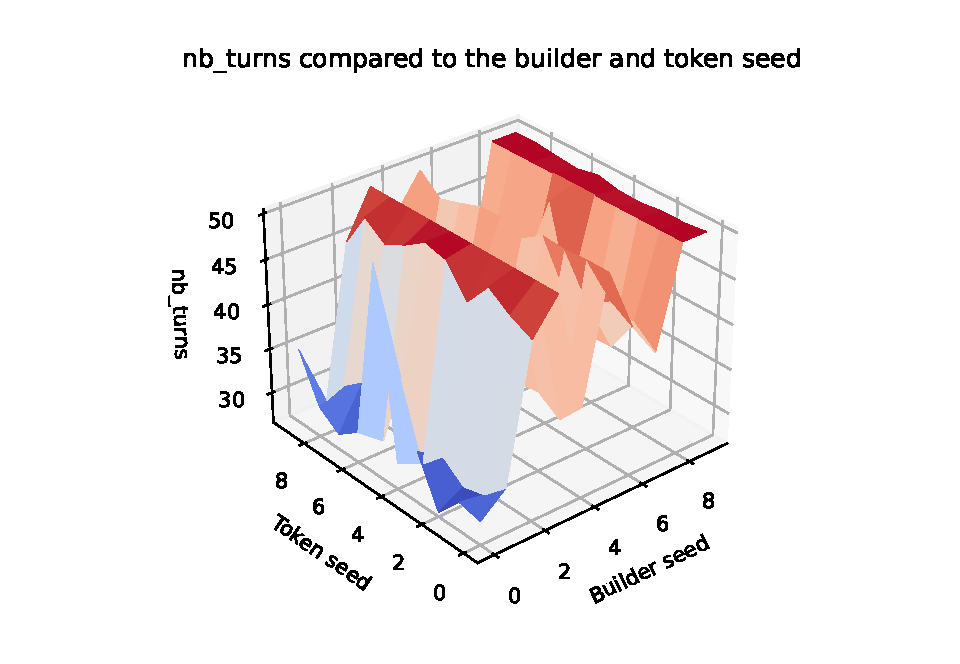
\includegraphics[width=\textwidth]{img/turns.pdf}
    \end{subfigure}
    \begin{subfigure}[b]{0.3\textwidth}
        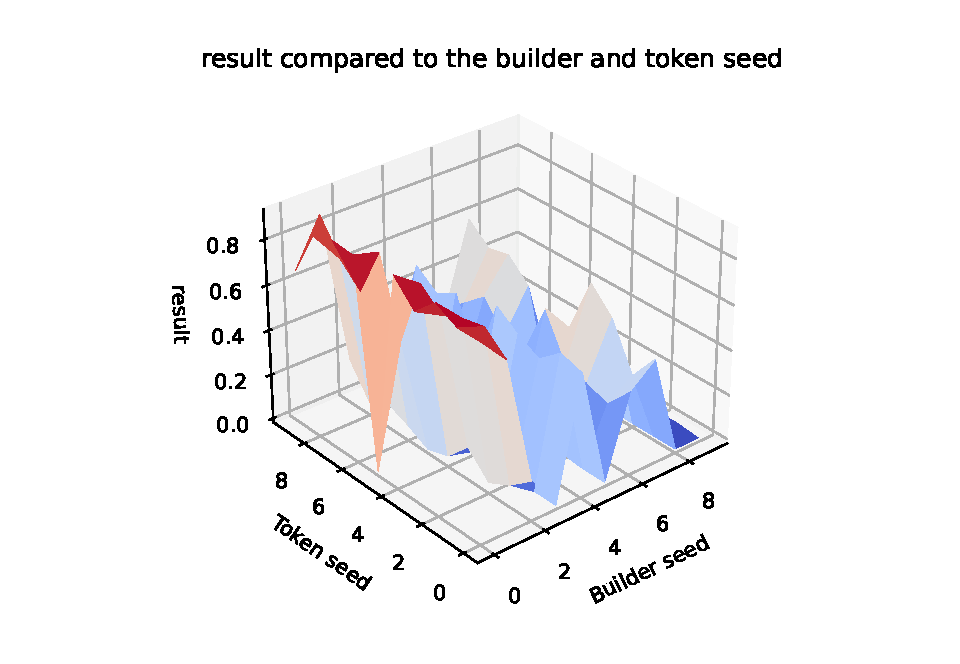
\includegraphics[width=\textwidth]{img/result.pdf}
    \end{subfigure} 
    \caption{Influence des graines sur différents paramètres de la partie}
\end{figure}

Précision : la graine 0 n'est pas générée aléatoirement mais correspond à un deck généré à la main afin d'avoir un jeu équilibré (selon nous).

A partir de ces graphiques, on remarque un comportement intéressant, la graine des architectes à beaucoup plus d'influence sur la viabilité de la partie (beaucoup de tour et pas trop de tour passés) que celle des jetons. Par exemple on voit que les joueurs sont forcés à passer souvent leur tour avec la graine d'architecte n°6 car il y a seulement 2 architectes de générés dans cette dernière.